\documentclass[12pt,a4paper]{article}
\usepackage[portuguese]{babel}
\usepackage[utf8]{inputenc}
\usepackage{microtype}
\usepackage{amsfonts}
\usepackage{amsthm}
\usepackage{graphicx}

\newcommand{\dpar}[1]{\left(#1\right)}

\newcommand{\N}{\mathbb{N}}
\newcommand{\R}{\mathbb{R}}

\theoremstyle{definition}
\newtheorem{ex}{Exercício}

\date{}

\begin{document}
\section*{Física geral 1: Lista 1}

\begin{ex}
  A posição de uma partícula em metros é dada pela expressão
  $x(t)=2t^3-6$, onde $t$ é medido em segundos. (i) Encontre a
  velocidade média da partícula entre os instantes $1\,\mathrm{s}$ e
  $2\,\mathrm{s}$. (ii) Determine a velocidade da partícula no
  instante $t=2\,\mathrm{s}$. \emph{Resposta:} (i) $14\,\textrm{m/s}$,
  (ii) $24\,\mathrm{m/s}$.
\end{ex}

\begin{ex}
  A velocidade de uma partícula em m/s é dada por $v(t)=10-5t$, onde
  $t$ é medido em segundos. Calcule o delocamento da partícula entre
  os instantes $1\,\mathrm{s}$ e $2\,\mathrm{s}$. \emph{Resposta:}
  $2{,}5\,\mathrm{m}$.
\end{ex}

\begin{ex}
  Considerando o gráfico $x$ vs $t$ dado na figura, responda as
  seguintes perguntas:
  \begin{enumerate}
  \item[(i)] Quais são os sinais possíveis para a velocidade da
    partícula entre os instantes $4\,\mathrm{s}$ e $6\,\mathrm{s}$?
  \item[(ii)] No instante $3\,\mathrm{s}$, a partícula está se movendo
    para a direita?
  \item[(iii)] A partícula volta para a sua posição inicial em algum
    instante? Qual?
  \item[(iv)] Quais são os possíveis sinais da aceleração da partícula
    entre os instantes $4\,\mathrm{s}$ e $6\,\mathrm{s}$?
  \item[(v)] Qual é a a velocidade da partícula no primeiro instante
    em que ela passa pela posição $2\,\mathrm{m}$? Qual é o sinal da
    sua aceleração?
  \end{enumerate}
  \begin{figure}[ht]
    \centering
    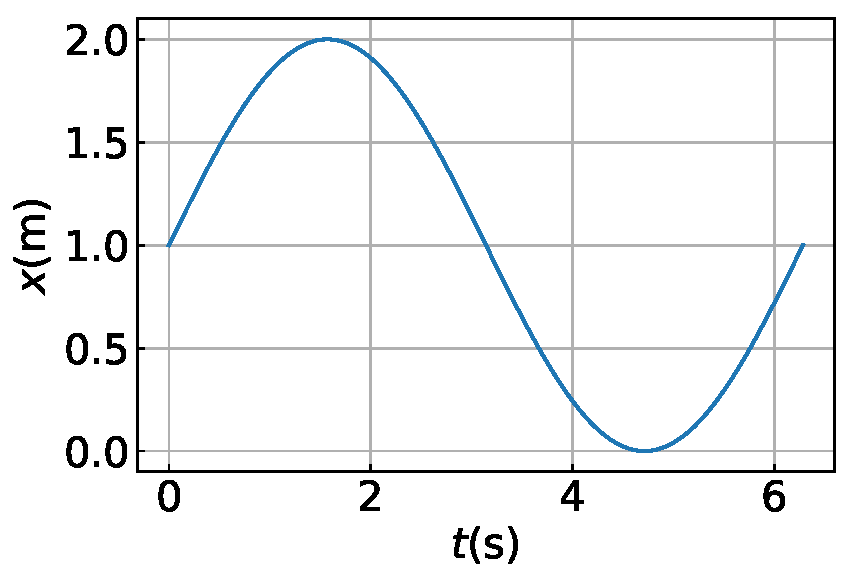
\includegraphics[width=0.5\textwidth,keepaspectratio]{xtcurve.pdf}
    \caption{Gráfico $x$ vs $t$.}
    \label{fig:xvst}
  \end{figure}
\end{ex}

\end{document}
